\subsection{Эллипс}
\textbf{Эллипс} --- плоская замкнутая кривая, сумма расстояний от любой точки котрой до двух фиксированных точек, называемых фокусами, постоянна и равна удвоенной большой полуоси эллипса.
$$F_1M+F_2M=const=2a$$
Главные отрезки эллипса:
\begin{enumerate}
\item Большая полуось ($a$)
\item Малая полуось ($b$)
\item Фокусное расстояние ($c$)
\end{enumerate}
$a$, $b$ и $c$ связаны слейдующим образом: $b^2+c^2=a^2$, что несложно вывести из определения эллипса.
 Эксцентриситет ($e$) --- числовая характеристика, показывающая степень отклонения от окружности. В эллипсе $0<e<1$.
 \begin{center}
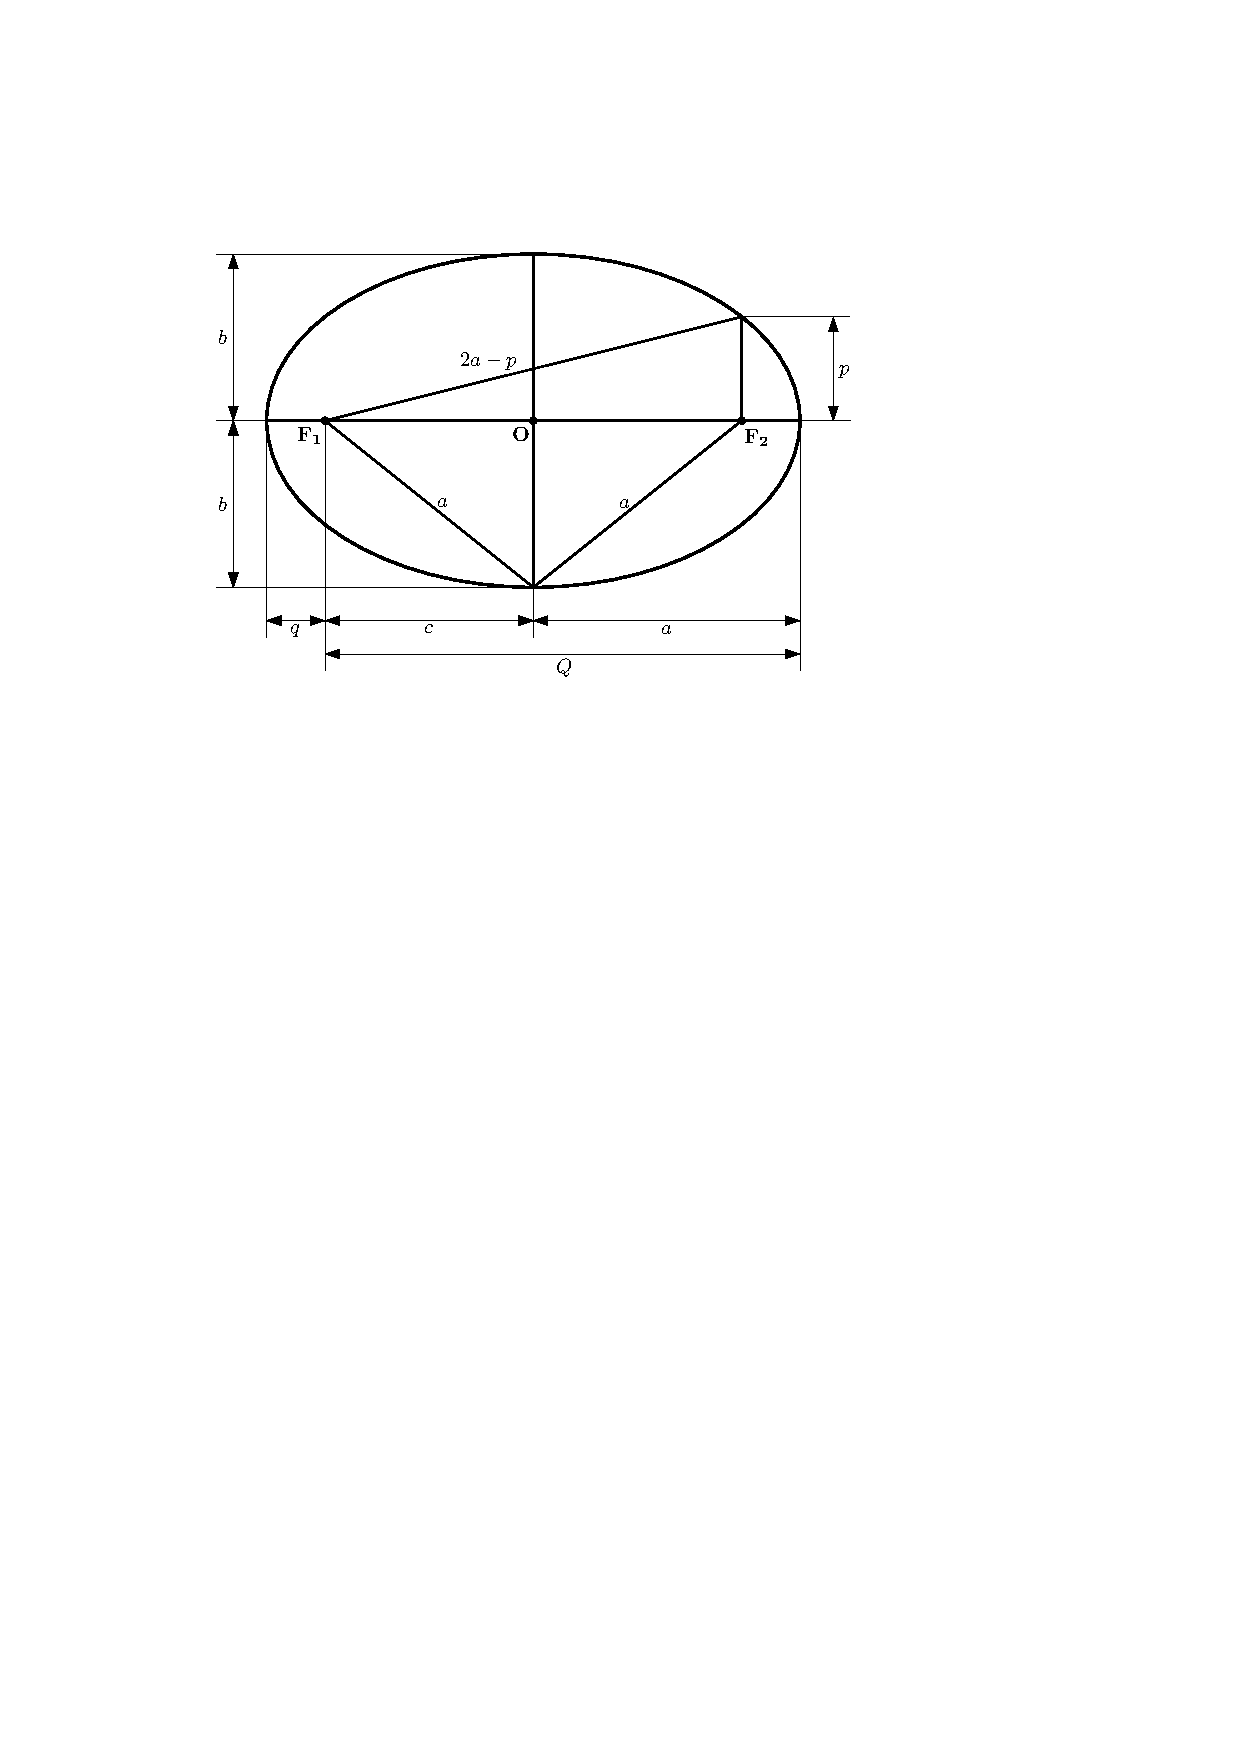
\includegraphics[width = 0.8\textwidth]{Ellips}
\begin{figure}[h!]
\caption{Эллипс}
\end{figure}
\end{center}
